\documentclass[a4paper, top=10mm]{article}
\usepackage[french]{babel}
%for writing from the top
\usepackage{fullpage}
%for math
\usepackage{amsmath}
\usepackage{mathrsfs}
\usepackage{amsthm}
%for images
\usepackage{graphicx}
%for color
\usepackage{xcolor}
%for title
\title{\textbf{\huge{Un rébus...}}}
\author{Enigme n\textsuperscript{o}4}
\date{20 Janvier 2024}

\newtheorem*{hint}{Hint}

\addtolength{\voffset}{-2cm}
\addtolength{\textheight}{5cm}


\begin{document}
	\maketitle
	
	\huge
	Résolvez le rébus suivant:
	
	\vspace{1cm}
	
	\begin{center}
		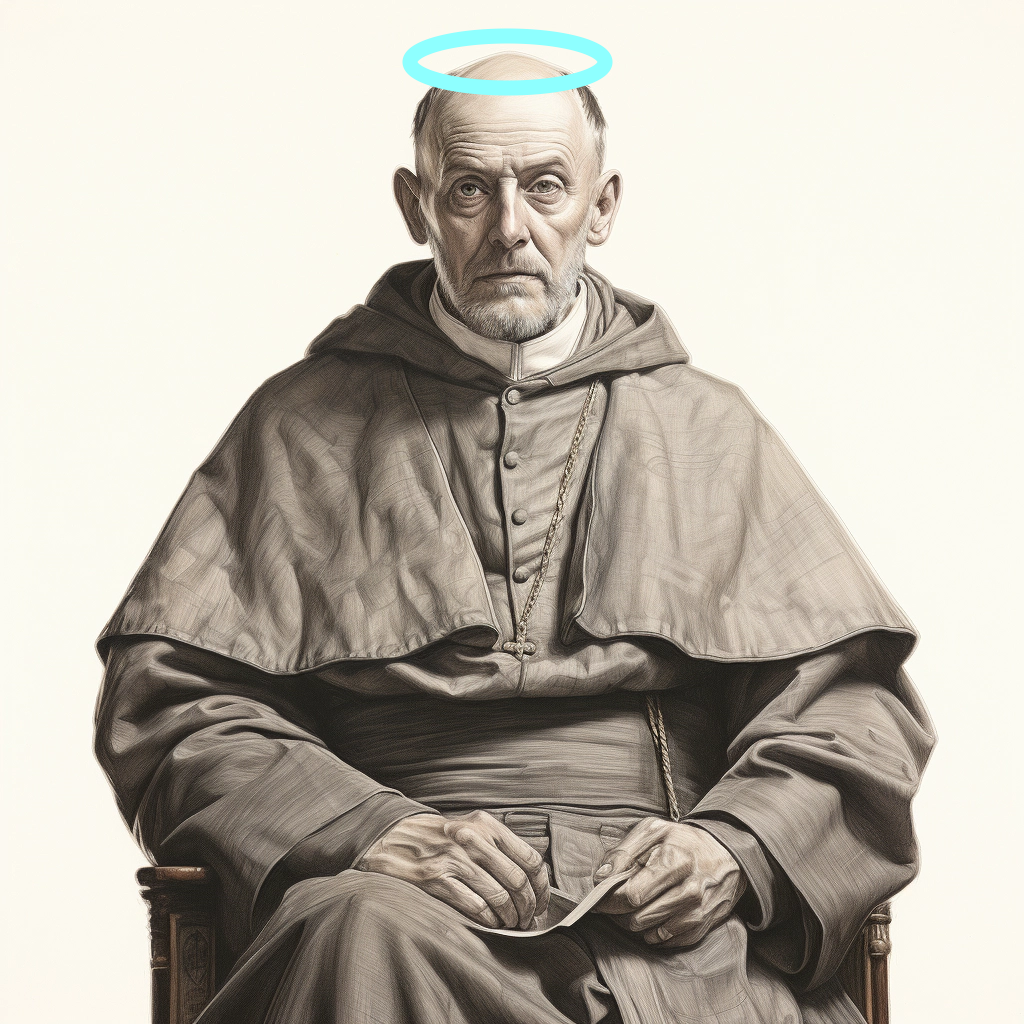
\includegraphics[width=200pt]{04saint.png}
		
\includegraphics[width=200pt]{04quand.png}\\
		\vspace{0.2cm}
		\hspace{1cm}
		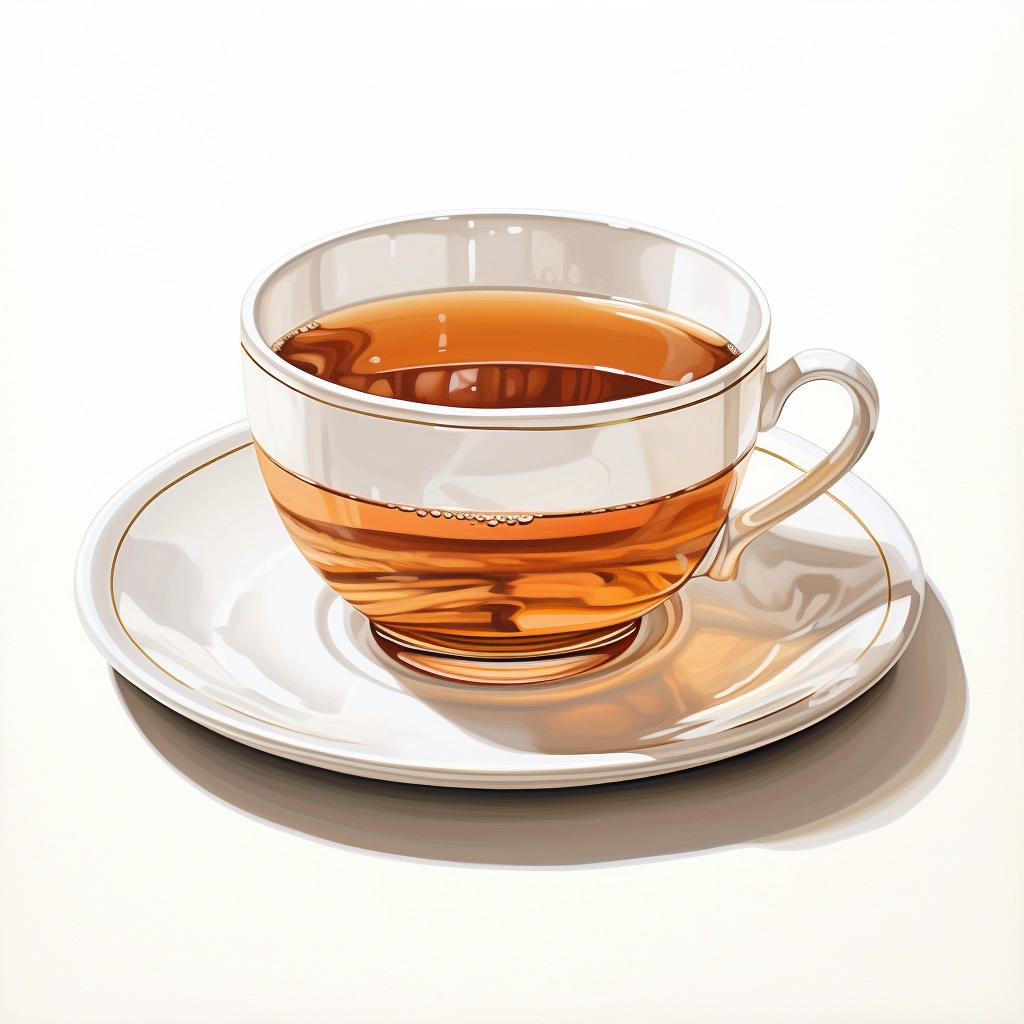
\includegraphics[width=200pt]{04the.png}
		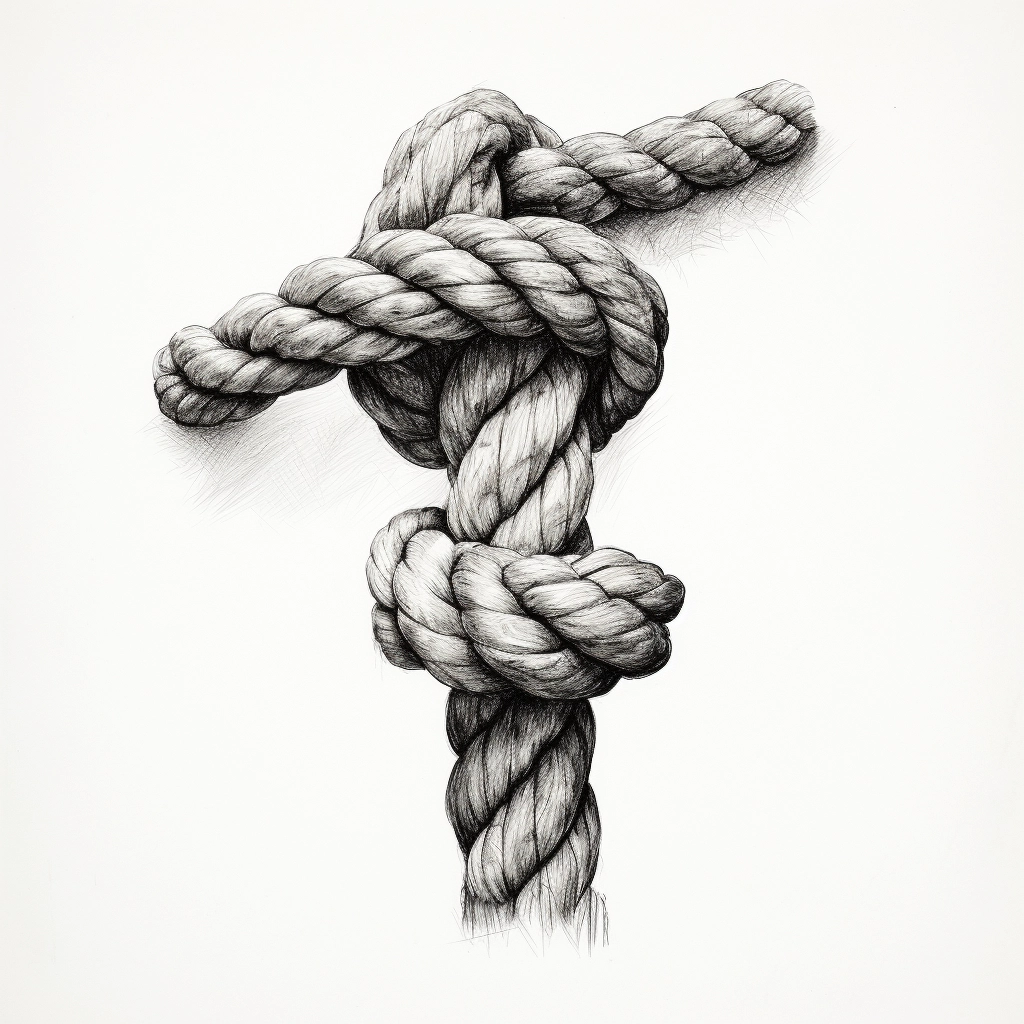
\includegraphics[width=200pt]{04node.png}
	\end{center}
	
\end{document}